%设置计数器为0
\setcounter{chapter}{0}
\chapter{}

\section{Feb 24 ex8.1:6,9,10,12,14,17,23,26.}

\begin{exercise}{8.1.6}
    设$\a,\b,\c$是满足$\a + \b + \c =\mathbf{0}$的单位向量,试求$\a \cdot \b + \b \cdot \c + \c \cdot \a$的值.
\end{exercise}

\begin{solution}
    由
    $$
    (\a + \b + \c) \cdot (\a + \b + \c) = \a \cdot \a + \b \cdot \b + \c \cdot \c + 2(\a \cdot \b + \b \cdot \c + \c \cdot \a) = 0,
    $$可得
    $$
    \a \cdot \b + \b \cdot \c + \c \cdot \a = -\frac{1}{2}(\a \cdot \a + \b \cdot \b + \c \cdot \c) = -\frac{3}{2}.
    $$
\end{solution}

\begin{exercise}{8.1.9}
    已知向量$\a$和$\b$的夹角$\theta = \frac{2 \pi}{3}$,又$|\a| = 1,|\b| = 2$,试计算:
    \begin{multicols}{2}
        \begin{enumerate}
            \item $|\a \times \b|^2$;
            \item $|(\a + 3\b) \times (3\a -\b)|^2$.
        \end{enumerate}
    \end{multicols}
\end{exercise}

\begin{solution}
    \begin{enumerate}
        \item $|\a \cdot \b|^2 = |\a|^2|\b|^2\cos^2\theta = 1$ , $|\a \times \b|^2 = |\a|^2|\b|^2\sin^2\theta = 3$.
        \item $|(\a + 3\b) \times (3\a -\b)|^2 = |3\a \times \a + 9\b \times \a - \a \times \b - 3 \b \times \b|^2 = |-10 \a \times \b|^2 = 100|\a \times \b|^2 = 300$.
    \end{enumerate}
\end{solution}

\begin{exercise}{8.1.10}
    已知$\a + \b + \c = \mathbf{0}$,试证$$\a \times \b = \b \times \c = \c \times \a.$$
\end{exercise}

\begin{solution}
    $$\a + \b + \c = \mathbf{0} \Rightarrow - \b = \a + \c \Rightarrow 0 = - \b \times \b = (\a + \c) \times \b = \a \times \b + \c \times \b \Rightarrow \a \times \b = - \c \times \b = \c \times \a.$$
\end{solution}

\begin{exercise}{8.1.12}
    求证: $|\a \times \b |^2 = |\a|^2|\b|^2 - (\a \cdot \b)^2$.
\end{exercise}

\begin{solution}
    $$
    |\a \times \b|^2 = \left( |\a||\b| \sin \theta \right)^2 = |\a|^2|\b|^2\sin^2\theta = |\a|^2|\b|^2 - |\a|^2|\b|^2\cos^2\theta = |\a|^2|\b|^2 - (\a \cdot \b)^2.
    $$
\end{solution}

\begin{exercise}{8.1.14}
    已知$\a = (3,-5,8), \b = (-1,1,-4)$,求$\a - \b$的模和方向余弦.
\end{exercise}

\begin{solution}
    $\a - \b = (4,-6,12)$, $|\a - \b| = 14$,
    $$
    \cos \alpha = \frac{4}{14} = \frac{2}{7}, \quad  \cos \beta = \frac{-6}{14} = -\frac{3}{7}, \quad \cos \gamma = \frac{12}{14} = \frac{6}{7}.
    $$
\end{solution}

\begin{example}{8.1.17}
    已知$\overrightarrow{OA} = 2 \i +4\j + \k, \overrightarrow{OB} = 3\i + 7\j + 5\k, \overrightarrow{OC} = 4\i + 10\j + 9\k$,问$A,B,C$是否共线?
\end{example}

\begin{solution}
    $\overrightarrow{OA} + \overrightarrow{OC} = 6 \i + 14 \j + 10 \k = 2\overrightarrow{OB}$,故$A,B,C$共线.
\end{solution}

\begin{exercise}{8.1.23}
    已知点$A(1,2,0),B(3,0,-3),C(5,2,6)$,求三角形$ABC$的面积.
\end{exercise}

\begin{solution}
    $\overrightarrow{AB} = 2\i - 2\j - 3\k, \overrightarrow{AC} = 4\i + 6 \k,$,故
    $$
    S = \frac{1}{2}|\overrightarrow{AB} \times \overrightarrow{AC}| = \frac{1}{2}|\begin{vmatrix}
        \i & \j & \k \\
        2 & -2 & -3 \\
        4 & 0 & 6
    \end{vmatrix}| = 14.
    $$
\end{solution}

\begin{exercise}{8.1.26}
    下列四点:$A(1,2,-1),B(0,1,5),C(-1,2,1),D(2,1,3)$.是否在一个平面上.
\end{exercise}

\begin{solution}
    $\overrightarrow{AB} = -\i - \j + 6\k, \overrightarrow{AC} = -2\i + 2\k, \overrightarrow{AD} = \i - \j + 4\k$,计算以$AB,AC,AD$为棱的平行六面体的体积为:
    $$
    V = |\overrightarrow{AB} \cdot (\overrightarrow{AC} \times \overrightarrow{AD})| = 
    \begin{vmatrix}
        -1 & -1 & 6 \\
        -2 & 0 & 2 \\
        1 & -1 & 4
    \end{vmatrix} = 0,
    $$故$A,B,C,D$在一个平面上.
\end{solution}

\section{Feb 26 ex8.2:1,2,3,6,7,14(1),15(1),16}

\begin{exercise}{8.2.1}
    指出下列平面位置的特点,并作图.\begin{multicols}{2}
        \begin{enumerate}
            \item $2x - 2y + 2z = -1$;
            \item $2x - 3y + 2 = 0$;
            \item $y-3z = 0$;
            \item $3x -2 = 0$.
        \end{enumerate}
    \end{multicols}
    
\end{exercise}

\begin{solution}
    \begin{enumerate}
        \item $2x - 2y + 2z =-1$ 与$Ox,Oy,Oz$轴的夹角角度相等,与$Oxy,Oyz,Ozx$平面的夹角角度相等.
        \item $2x - 3y + 2 = 0$ 与$Oz$轴平行,与$Oxy$平面垂直;
        \item $y - 3z = 0$ 与$Ox$轴平行,与$Oyz$平面垂直;
        \item $3x - 2 = 0$ 与$Ozy$平面平行,与$Ox$轴垂直.
    \end{enumerate}

    \begin{figure}[htbp]
      \centering
      \begin{subfigure}{0.23\textwidth}
        \centering
        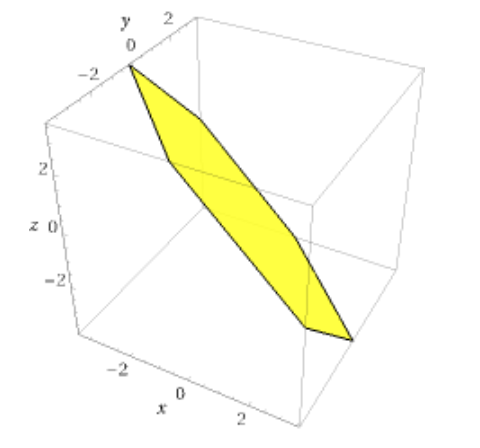
\includegraphics[width=\linewidth]{figure/1-3.png}
      \end{subfigure} \hfill
      \begin{subfigure}{0.23\textwidth}
        \centering
        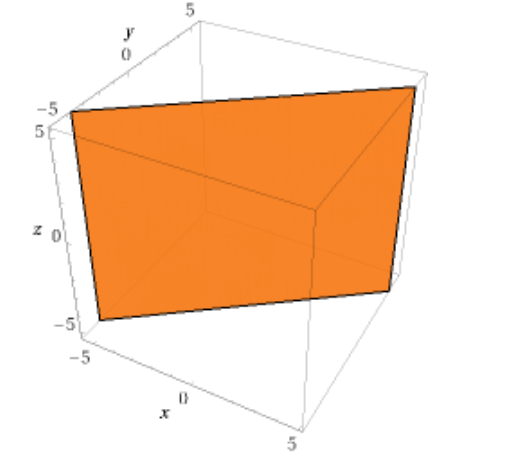
\includegraphics[width=\linewidth]{figure/1-4.png}
      \end{subfigure} \hfill
      \begin{subfigure}{0.23\textwidth}
        \centering
        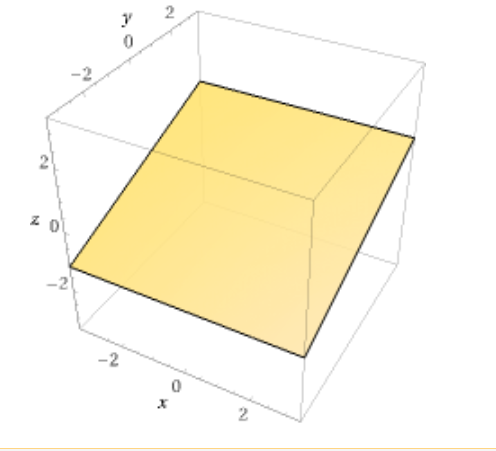
\includegraphics[width=\linewidth]{figure/1-5.png}
      \end{subfigure} \hfill
      \begin{subfigure}{0.23\textwidth}
        \centering
        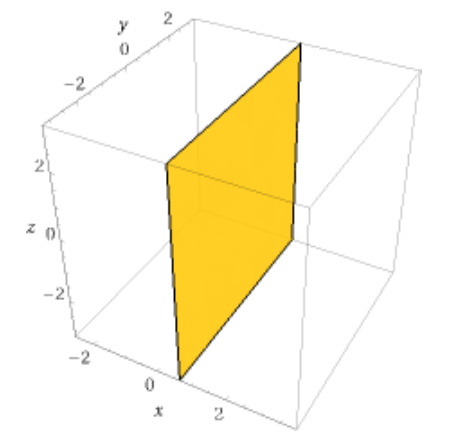
\includegraphics[width=\linewidth]{figure/1-6.png}
      \end{subfigure}
      \caption{习题 8.2.1}
    \end{figure}
\end{solution}

\begin{exercise}{8.2.2}
    试求通过点 $M_1(2, -1, 3)$ 和 $M_2(3, 1, 2)$ 且平行于向量 $\v = (3, -1, 4)$ 的平面方程.

\end{exercise}

\begin{solution}
    (法一)

    平面平行于$\overrightarrow{M_1M_2} = (1, 2, -1), \v = (3, -1, 4)$,故平面的一个法向量为$\overrightarrow{M_1M_2} \times \v = (1,-1,-1)$,故平面方程可以写为
    $$
    x - y - z = D.
    $$
    代入$M_1$得$D = 0$,故平面方程为$x - y - z = 0$.

    (法二)
    设平面方程为 $ ax + bx + c + d = 0 $,则

\[
\left\{
\begin{aligned}
2a - b + 3c + d = 0 \\
3a + b + 2c + d = 0 \\
3a - b + 4c = 0
\end{aligned}
\right.
\quad \Rightarrow \quad
\left\{
\begin{aligned}
a + c = 0 \\
b = c \\
d = 0
\end{aligned}
\right.
\]

故平面方程为 $x - y - z = 0$.

\end{solution}

\begin{exercise}{8.2.3}
    设平面过点 $(5, -7, 4)$ 且在 $x, y, z$ 三轴上的截距相等,求平面方程.
\end{exercise}

\begin{solution}
    设平面方程为$ Ax + By + Cz = D$.

    当$D = 0$时,平面过点$(5,-7,4)$,故$5A - 7B + 4C = 0$,解得$A =4t, B = 4s, C = -5t+7s$,平面方程有无穷多个,形如$4tx + 4sy - (5t - 7s)z = 0$,其中$t,s$为任意实数.

    当$D \neq 0 $时,截距相等推出平面的一个法向量为$(1,1,1)$,代入点$(5,-7,4)$,得平面方程为
    $$
    x + y + z = 2.
    $$
\end{solution}

\begin{exercise}{8.2.6}
    求通过点 $ M(-5, 2, -1) $ 且平行于坐标平面 $ Oyz $ 的平面方程.
\end{exercise}

\begin{solution}
    平行于坐标平面$Oyz$,故目标平面的一个法向量为$(1,0,0)$,设平面方程为$Ax+D=0$,代入$M$点即得平面方程为
    $$
    x = -5.
    $$
\end{solution}

\begin{exercise}{8.2.7}
    求下列各平面的夹角:
\begin{enumerate}
  \item $ 2x - y + z - 7 = 0 $ 和 $ x + y + 2z - 11 = 0 $;
  \item $ 4x + 2y + 4z - 7 = 0 $ 和 $ 3x - 4y = 0 $.
\end{enumerate}
\end{exercise}

\begin{solution}
    \begin{enumerate}
        \item 法向量 $ \mathbf{n_1} = (2, -1, 1), \ \mathbf{n_2} = (1, 1, 2) $,因此
        \[
        \theta = \arccos\left( \frac{\mathbf{n_1} \cdot \mathbf{n_2}}{|\mathbf{n_1}| |\mathbf{n_2}|} \right) = \arccos\left( \frac{1}{2} \right) = \frac{\pi}{3}
        \]
        \item 法向量 $ \mathbf{n_1} = (2, 1, 2), \ \mathbf{n_2} = (3, -4, 0) $,因此
        \[
        \theta = \arccos\left( \frac{\mathbf{n_1} \cdot \mathbf{n_2}}{|\mathbf{n_1}| |\mathbf{n_2}|} \right) = \arccos\left( \frac{2}{15} \right)
        \]
    \end{enumerate}
\end{solution}

\begin{exercise}{8.14.(1)}
    分别按下列各组条件求平面方程.
\begin{enumerate}
  \item 平分两点 $ A(1, 2, 3) $ 和 $ B(2, -1, 4) $ 之间的线段且垂直于线段 $ AB $;
\end{enumerate}
\end{exercise}

\begin{solution}
    该平面有法向量 $ \overrightarrow{AB} = (1, -3, 1) $,因此,可设方程为 $ x - 3y + z + d = 0 $.再带入中点 $ \left( \frac{3}{2}, \frac{1}{2}, \frac{7}{2} \right) $,得到
\[
2x - 6y + 2z - 7 = 0
\]
\end{solution}

\begin{exercise}{8.15.(1)}
    分别求出满足下列各条件的直线方程.
\begin{enumerate}
    \item 过点 $ (0, 2, 4) $ 且与平面 $ x + 2z = 1, \ y - 3z = 2 $ 平行;
\end{enumerate}
\end{exercise}

\begin{solution}
    两平面的法向量为 $ \mathbf{n_1} = (1, 0, 2), \mathbf{n_2} = (0, 1, -3) $,则
\[
\mathbf{n_1} \times \mathbf{n_2} = (-2, 3, 1)
\]
设直线的参数方程为$(x,y,z) = (x_0,y_0,z_0) + (-2,3,1)t$,代入点$(0,2,4)$可解出$x_0=0,y_0=2,z_0=4$.
因此直线方程为
\[
(x, y, z) = (0, 2, 4) + (-2, 3, 1)t
\]
\end{solution}

\begin{exercise}{8.16}
    求直线
\[
\left\{
\begin{aligned}
  2x + 3y - z - 4 &= 0, \\
  3x - 5y + 2z + 1 &= 0
\end{aligned}
\right.
\]
的参数方程.
\end{exercise}

\begin{solution}
    两平面的法向量为 $ \mathbf{n_1} = (2, 3, -1), \ \mathbf{n_2} = (3, -5, 2) $,则
\[
\mathbf{n_1} \times \mathbf{n_2} = (1, -7, -19)
\]
为其方向量.进一步,可求得直线上一点 $ (1, 0, -2) $.因此,参数方程为:
\[
\left\{
\begin{aligned}
x &= 1 + t \\
y &= -7t \\
z &= -2 - 19t
\end{aligned}
\right.
\]
或者写为
$$
(x,y,z) = (1,0,-2) + (1,-7,-19)t.
$$
\end{solution}

\section{Feb 28 ex8.2:18(1),19(1),20(2),21(1),22(1),23(1),29,30}

\begin{exercise}{ex8.2,18(1)}
    求下列直线的夹角:
    \begin{enumerate}
        \item $\begin{cases}
            5x - 3y + 3z - 9 = 0,\\
            3x -2y + z -1 = 0.
        \end{cases}$和$\begin{cases}
            2x + 2y -z +23 =0,\\
            3x + 8y + z -18 = 0.
        \end{cases}$
    \end{enumerate}
\end{exercise}

\begin{solution}
    两条直线的方向量分别为
\[
\bm{a} = (5, -3, 3) \times (3, -2, 1) = (3, 4, -1)
\]
\[
\bm{b} = (2, 2, -1) \times (3, 8, 1) = (10, -5, 10)
\]
因此夹角为
\[
\theta = \arccos \frac{\bm{a} \cdot \bm{b}}{|\bm{a}| |\bm{b}|} = \frac{\pi}{2}
\]
\end{solution}

\begin{exercise}{ex8.2,19(1)}
    证明下列各组直线互相平行,并求他们之间的距离.
    \begin{enumerate}
        \item $\frac{x+2}{-2} = \frac{y-1}{3} = -z$和$\begin{cases}
            x+y+z = 0,\\
            x-y-5z-8=0.
        \end{cases}$
    \end{enumerate}
\end{exercise}

\begin{solution}
    两条直线的方向向量分别为
    $$\a = (-2,3,-1)$$和
    $$\b = (1,1,1) \times (1,-1,-5) = (-4,6,-2).$$ 
    两方向向量平行,故两直线平行.

    两直线各取一点$M(-2,1,0),N(4,-4,0)$,则两直线距离为
    $$
    d = \frac{|\overrightarrow{MN} \times \a |}{| \a |} = \frac{|(5,6,8)|}{|(-2,3,-1)|} = \sqrt{\frac{125}{14}}
    $$
\end{solution}

\begin{exercise}{8.2.20(2)}
    证明下列各组直线垂直相交,并求它们的交点.
    \begin{enumerate}
        \item $\begin{cases}
            4x+y-3z+24=0,\\
            z-5=0.
        \end{cases}$和$\begin{cases}
            x+y+3=0.\\
            x+2.
        \end{cases}$
    \end{enumerate}
\end{exercise}

\begin{solution}
    两条直线的方向量分别为
\begin{align*}
    & \bm{a} = (4, 1, -3) \times (0, 0, 1) = (1, -4, 0)\\
    & \bm{b} = (1, 1, 0) \times (1, 0, 0) = (0, 0, -1).
\end{align*}
得到 $\bm{a} \cdot \bm{b} = 0$,因此垂直.
进一步,联立两个方程式,存在交点 $(-2, -1, -5)$.
\end{solution}

\begin{exercise}{8.2.21(1)}
     求直线和平面的夹角 $\varphi$.
        
        \begin{enumerate}
            \item 
            $
            \left\{
            \begin{aligned}
            3x - 2y &= 24, \\
            3x - z &= -4,
            \end{aligned}
            \right.$
            \quad $6x + 15y - 10z + 31 = 0;$
        \end{enumerate}
\end{exercise}

\begin{solution}
    直线的方向向量为
\[
\bm{a} = (3, -2, 0) \times (3, 0, -1) = (2, 3, 6)
\]
平面的法向量为 $\bm{n} = (6, 15, -10)$,因此夹角为
\[
\varphi = \arccos \frac{|\bm{a} \cdot \bm{n}|}{|\bm{a}|} = \arcsin \frac{3}{133}.
\]
\end{solution}


\begin{exercise}{8.2.22(1)}
    求点到直线的距离 $d$.
    
    \begin{enumerate}
        \item $P_0(1, 0, -1), \quad \frac{x}{1} = \frac{y-1}{2} = \frac{z}{-1};$
    \end{enumerate}
    \end{exercise}

\begin{solution}
    直线的方向向量为 $\bm{a} = (1, 2, -1)$.取直线上的点 $P(0, 1, 0)$,则线段 $PP_0$ 在直线上的投影长为
\[
\left|\frac{\overrightarrow{PP_0} \cdot \bm{a}}{|\bm{a}|}\right| = 0.
\]
因此 $PP_0$ 就是垂线段,长度为 $\left| \overrightarrow{PP_0} \right| = \sqrt{3}$.
\end{solution}

\begin{exercise}{8.2.23(1)}
    
\end{exercise}

\begin{exercise}
证明下列各直线是异面直线,并求它们的距离(即两直线垂线长).

\begin{enumerate}
    \item $\frac{x - 9}{4} = \frac{y + 2}{-3} = \frac{z}{1}$和$\frac{x}{-2} = \frac{y+7}{9} = \frac{z-2}{2}$;
\end{enumerate}
    \end{exercise}
    
    \begin{solution}
    两直线的方向向量分别为$\a = (4,-3,1), \b = (-2,9,2)$,分别取两直线上一点$A(9, -2, 0), B(0, -7, 2)$,
    \[
    \bm{a} \times \bm{b} \cdot \overrightarrow{AB} = 245 \neq 0
    \]
    知两直线异面.
    因此,两直线距离为
    \[
    d = \frac{|\bm{a} \times \bm{b} \cdot \overrightarrow{AB}|}{|\bm{a} \times \bm{b}|} = 7.
    \]
    \end{solution}

\begin{exercise}{8.2.29}
求原点关于平面 $6x + 2y - 9z + 121 = 0$ 对称的点的坐标.
\end{exercise}

\begin{solution}
    设对称点为$O'$,则$\overrightarrow{OO'} \perp \pi:6x+2y-9z$,故$\overrightarrow{OO'}$平行于平面的法向量$(6,2,-9)$,故设$O' = (6t,2t,-9t)$.

    将中点坐标$(3t,t,-,\frac92 t)$代入平面方程,解得$t = -2$,因此对称点的坐标为$O'(-12,-4,18)$.
\end{solution}

\begin{exercise}{8.2.30}
求点 $(1, 2, 3)$ 关于直线 $\frac{x}{1} = \frac{y - 4}{-3} = \frac{z - 3}{-2}$ 对称的点的坐标.
\end{exercise}

\begin{solution}
    设所求点的坐标为 $(a, b, c)$,将它与 $(1, 2, 3)$ 连线的中点坐标代入直线方程,得到
\[
b = -3a + 3, \quad c = -2a + 1.
\]
直线的方向向量为 $(1, -3, -2)$,故进一步地有
\[
0 = (1, -3, -2) \cdot \left( (a, b, c) - (1, 2, 3) \right) = 14a \Rightarrow a = 0.
\]
因此所求对称点为 $(0, 3, 1)$.
\end{solution}
    





